\documentclass[german,english]{bvm2020}

%==============================================================================
%Dies ist die Finale Vorlage des Autorenkits
%Version von BVM-PLRI Team
%Dieser Kommentar darf nicht gelöscht werden
%Kontrollzeileabc
\def\type{ERROR} % wird w{\"a}hrend der Nachbearbeitung und NICHT DURCH DIE AUTOREN eingetragen: Beitragsart: ``V'' = Vortrag, ``P'' = Poster, ``S'' = Softwaredemonstration

%==============================================================================
% Bitte tragen Sie hier anstelle von 0000 die Nummer Ihres Beitrags ein
\def\articlenumber{0000}

%==============================================================================
\date{}
%==============================================================================
% definieren Sie im Befehl \title den Titel Ihres Proceedings
%
\title{Refining multi-organ segmentation using partially annotated datasets
}
\def\titlefuertoc{Bildverarbeitung f\"ur die Medizin}

%==============================================================================
% sollte der Titel Ihres Proceedings in der Kopfzeile überstehen geben Sie 
% bitte mit dem Befehl \titelrunning eine Kurzform für die Kopfzeile an
%
%\titlerunning{Bildverarbeitung für die Medizin 2020}

%==============================================================================
% definieren Sie im Befehl \subtitle wenn gewünscht den Unteritel Ihres 
% Proceedings
%
%\subtitle{Richtlinien zur Erstellung der druckfertigen Beitr\"age}

%==============================================================================
% definieren Sie mit dem Befehl \author die beteiligten Autoren, trennen Sie 
% durch Kommata
% eine ~ anstelle eines Leerzeichen verhindert eine Trennung innerhalb des 
% Namens
% bei Beteiligung mehrerer Institute schreiben Sie die Nummer des Instituts 
% (s.u.) im Mathematikmodus hochgestellt direkt hinter den Namen
%
\author{Haobo~Song, Chang~Liu}
%\def\authorfuertoc{Thomas~M.~Deserno, Heinz~Handels, Andreas~Maier, Klaus~Maier-Hein, Christoph~Palm, Thomas~Tolxdorff}

%==============================================================================
% definieren sie mit dem Befehl \authorrunning die Liste der Autoren, wie sie 
% in der Kopfzeile erscheinen soll
% kürzen Sie dabei die Vornamen durch den ersten Buchstaben ab
% sollten mehr als 3 Autoren beteiligt sein führen Sie nur den Hauptautor 
% gefolgt von et al. auf
%
\authorrunning{Haobo~Song, Chang~Liu}
% bei weniger als 4 Autoren trennen Sie bitte wie im folgenden Beispiel
% \authorrunning{Author1, Author2 and Author3}

%==============================================================================
% definieren sie mit dem Befehl \institute entsprechend dem Beispiel die 
% beteiligten Institute
% jedes Institut folgt in einer neuen Zeile und bekommt seine Nummer (s.o.) im 
% Mathematikmodus vorrangestellt
%
\institute{%
$^1$Fakult\"at f\"ur Pattern Recognition, FAU Erlangen-N\"urnberg\\
}

%==============================================================================
% geben Sie mit dem Befehl \email die E-Mail-Adresse des korrespondierenden
% Autors an
%
\email{haobo.song@fau.de}

\begin{document}

%==============================================================================
% wählen Sie mit dem Befehl \selectlanguage die Sprache aus, in der Ihr 
% Proceeding verfasst ist
%
%\selectlanguage{german}
\selectlanguage{english}

\maketitle

\begin{abstract}
U-Net is a generic deep-learning solution for segmentation in biomedical image data. When training a new U-Net\cite{ronneberger2015unet} model for a specific segmentation task, getting finely-annotated datasets is usually difficult. In comparison to the method of training with a all-annotated dataset, we have verified a hypothesis. The model was trained by a series of partially annotated datasets with particular training method. 
\end{abstract}

\section{Introduction}
%
In the field of radiation therapy and CT dose optimization, segmentation of organs at risk in CT scanning is usually required to facilitate the treatment planning or dose estimation. The growing number of people choosing neural networks for segmentation tasks \cite{HAVAEI201718}. When developing deep learning multi-organ segmentation tools, dataset is usually a problem since getting manual segmentation of all organs from medical staff is usually very difficult. Meanwhile, there exist many publicly available datasets where not all required organs are annotated. The following table \ref{0001-tab-exper} illustrates some public partially annotated datasets on the internet.

\begin{table}[htbp]
	\caption{Partially annotated datasets source from the Internet}
	\label{0001-tab-exper}
	\begin{tabular*}{\textwidth}{l@{\extracolsep\fill}llllll}
		\hline
Source                    & Liver & Lung  & Brain & Cardiac & Kidney \\		\hline
Medicaldecathlon          & True  & True  & True  & True    & False \\
kits21                    & False & False & False & False   & True  \\
Cancerimagingarchive-Lung & False & True  & False & False   & False \\
Codalab                   & True  & False & False & False   & False	\\	\hline
\end{tabular*}
\end{table}
 However, simply mixing fully annotated dataset and partially annotated dataset can ‘spoil’ the training, because the partially annotated dataset can be considered falsely annotated and the convergence of the training is more difficult.

We offer an approach is that the ground truth  in the training step will be combined with the prediction from the model. Then the loss function is expected not to be biased by the missing annotations. Thus, the training can keep the performance for organs missing in partially annotated dataset, while improve the performance for organs in both fully and partially annotated dataset, since more training data is included. In the following section we explain the network architecture and analyse the result of experiments.




\section{Material and methods}
%
Our experiments is basis on U-Net and the experiment data are 3-D CT whole body volume. We need to modify the dataset and the training process in order to implement the algorithm. The dataset we need and the principles of the algorithm are described quickly below

\subsection{U-Net}
  U-Net is named after its U-shaped architecture. Since it was introduced, it has become a popular deep network architecture to deal with semantic segmentation \cite{Baheti_2020_CVPR_Workshops}. Due to the practicality of the network and the ability to learn from limited data. The following experiments is basis on U-Net.

\begin{SCfigure}[][htbp]
	\centering
	\label{u-net-architecture}
	\setlength{\figbreite}{0.5\linewidth}
	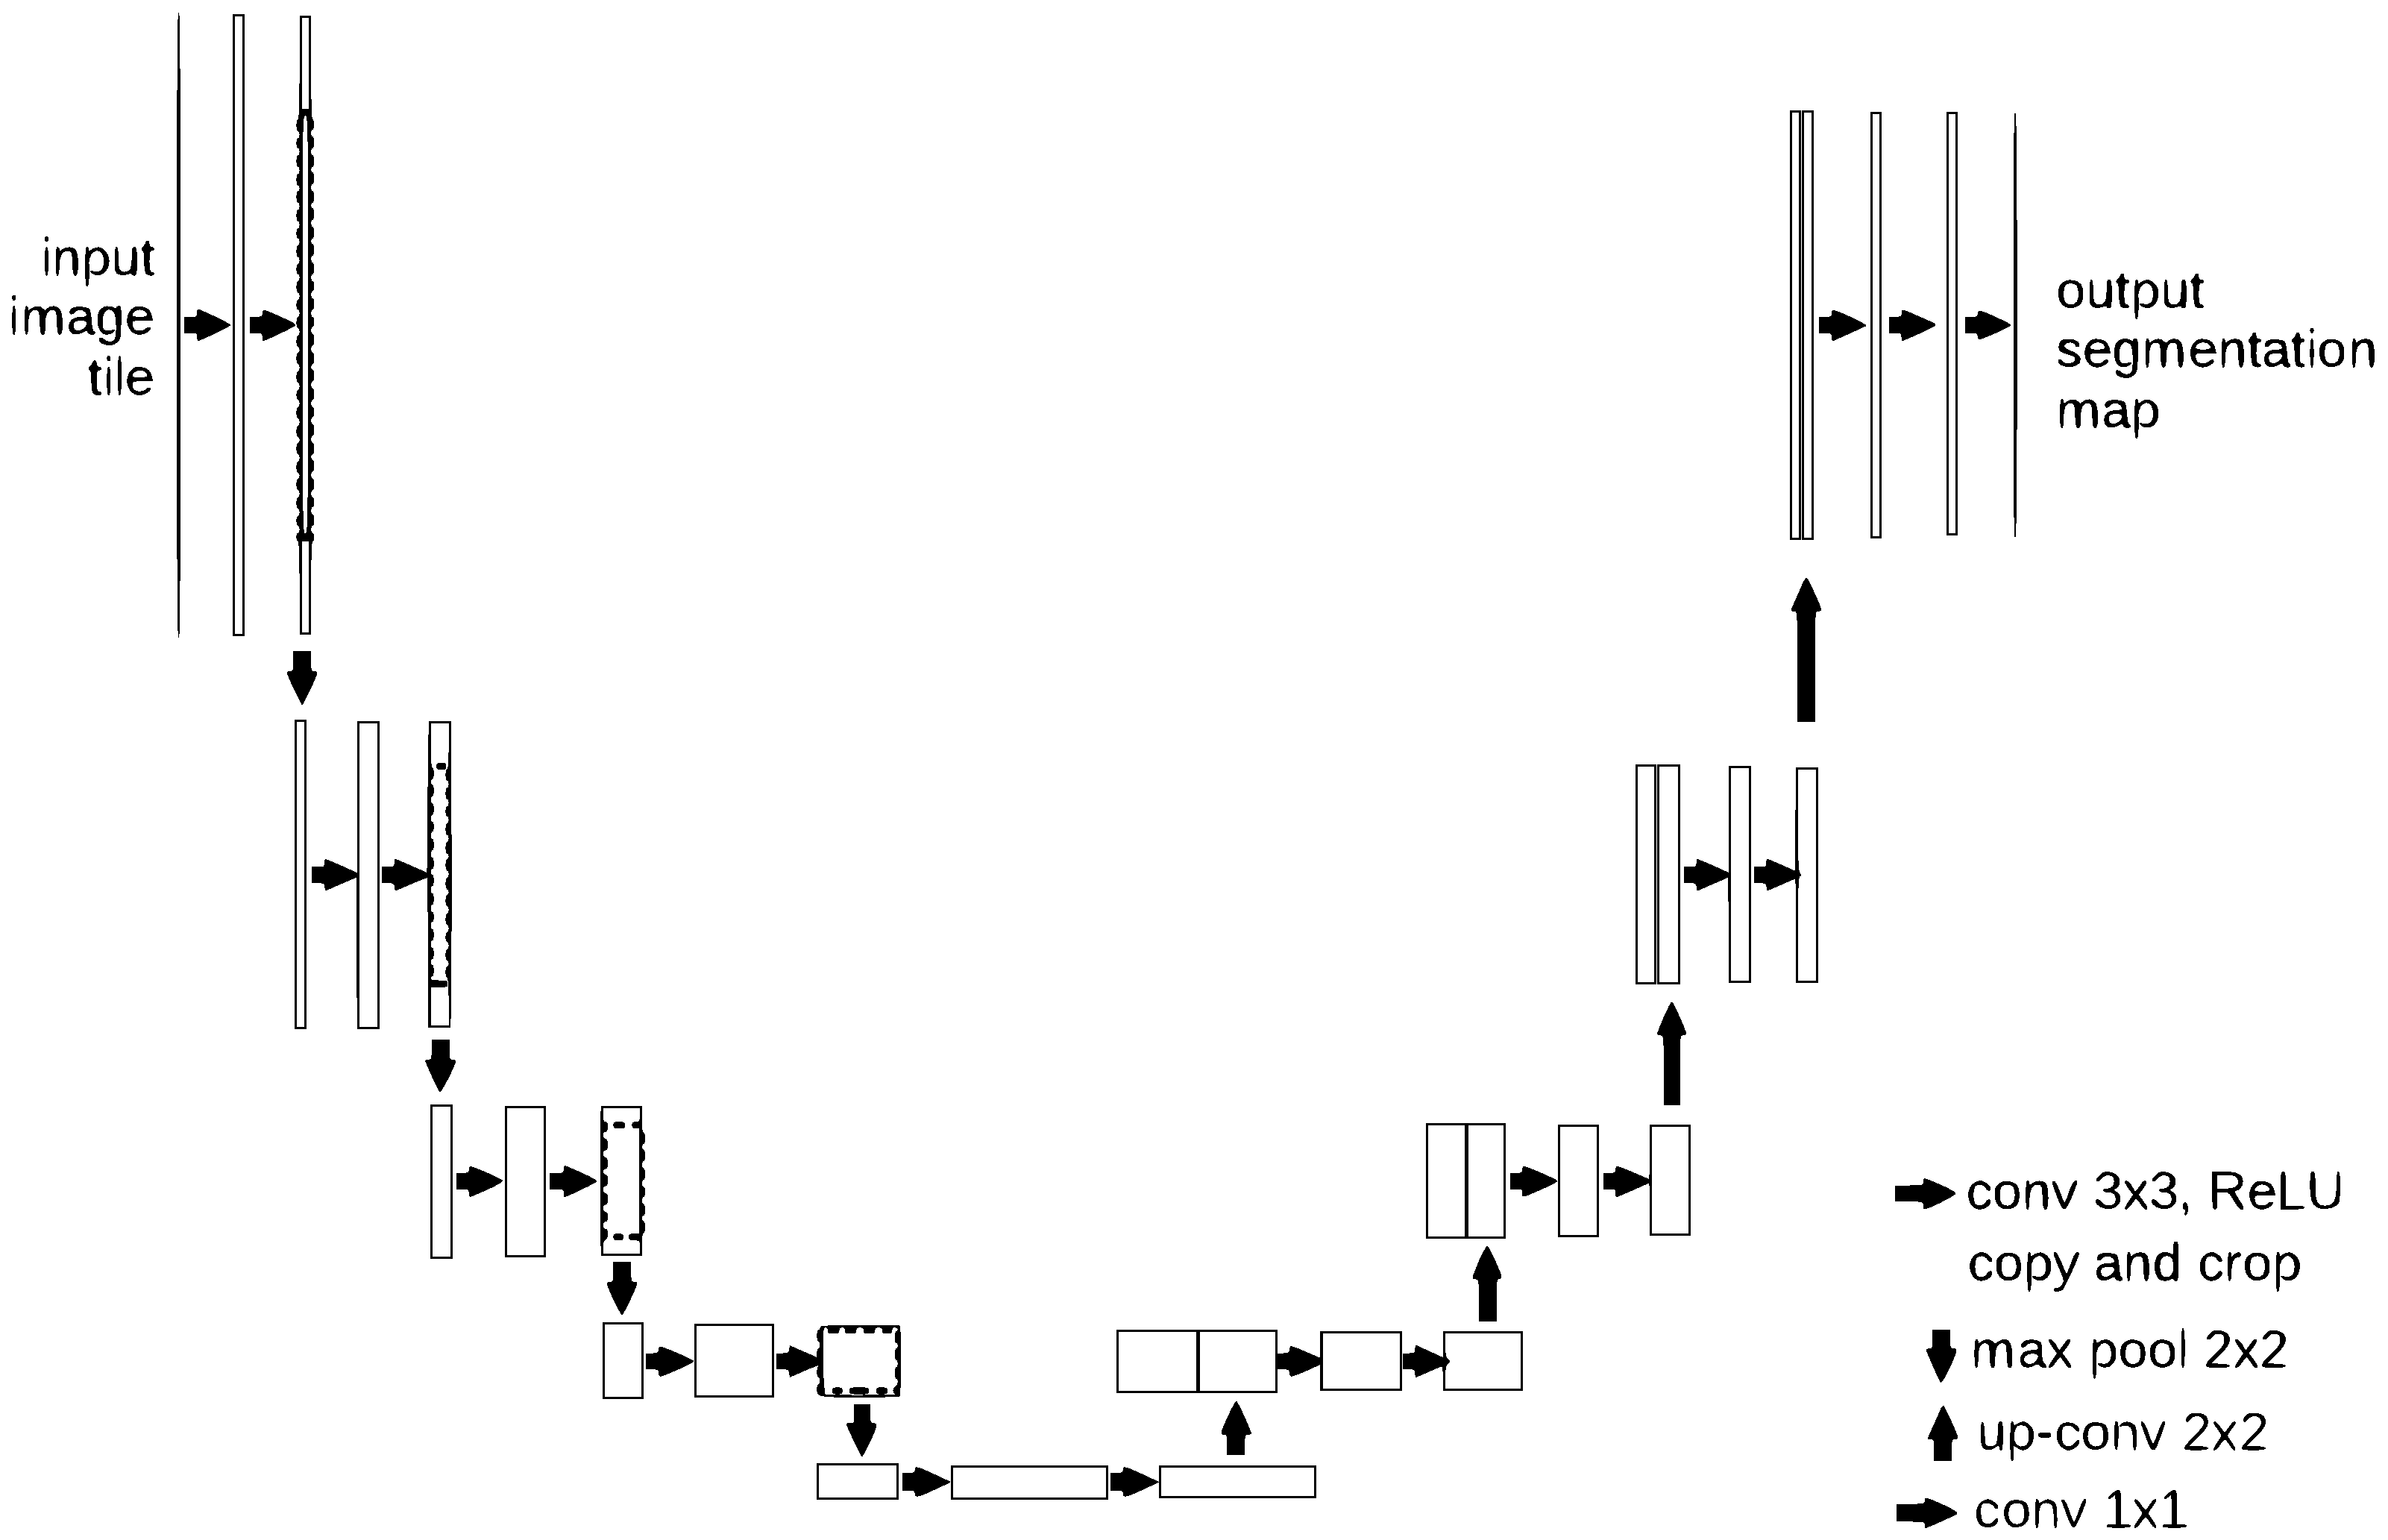
\includegraphics[width=\figbreite,height=\figbreite]{u-net-architecture}
	\caption{The architecture of U-Net\cite{ronneberger2015unet}}
\end{SCfigure}
The U-Net in the experiment was built according to the architecture diagram \ref{u-net-architecture} above, and the final output was one layer which size is 512*512 pixels and include labels: background(0), liver(1), right lung(2), and left lung(3)


\subsection{Dataset}
The dataset is from public xxxx and consists of 34 patients. Each patient has 400-500 CT full body scan 2D images with same pixel-spacing. These 2D images have zero-paded into the same size 512 * 512. In the following experiment, the different experimental group consisted of the corresponding number of patients. Furthermore, the original dataset is a fully annotated dataset, we have utilized masks to simulate the non-fully annotated dataset from fully annotated dataset. 
\begin{figure}[htbp]
	\setlength{\figbreite}{\textwidth}
	\centering
	\subfigure[Original Input]{\includegraphics[width=0.3\figbreite]{maskroi} 
	\label{fig-oi}}
	\subfigure[Original Label]{\includegraphics[width=0.3\figbreite]{maskgold}
		\label{fig-oo}}
	\subfigure[Modified Label]{\includegraphics[width=0.3\figbreite]{maskgnew}
		\label{fig-on}}
	\caption{Simulation of partially-labelled missing data sets by masking }
	\label{mask}
\end{figure}

As the image \ref{mask}  shows, There are three organs in original Input image \ref{fig-oi} that need to be segmented. At the beginning annotation data has three types of label, liver, right lung and left lung \ref{fig-oo}, after masking, the image has two types of annotation, the label of the right lung and left lung \ref{fig-on}. The reason for this is that the annotation belonging to the liver has been changed to background. while for the lungs annotation, it was retained. In this way a dataset without liver annotations was simulated.



\subsection{Modified training method}
Due to the dataset is composed of fully and partially annotated datasets. The training step should make some change to accommodate such special datasets. 
\begin{figure}[htbp]
	\setlength{\figbreite}{0.8\textwidth}
	\centering
	\includegraphics[width=\figbreite]{diagram}
	\caption{Process diagram of the training stage}
	\label{fig-diagram}
\end{figure}
From the figure \ref{fig-diagram} you can see that for the partial annotated data set we have changed the training method.The main idea is that predicted results intervene on the original label to reduce the impact of partially annotated data. The details of the algorithm for the new training step are as follows


\begin{algorithm} 
	\caption{New Train step} 
	\label{alg3} 
	\begin{algorithmic}
		\REQUIRE train data $input$, ground truth $target$
		\ENSURE modified ground truth $targetCopy$
		\STATE $pred \gets model(input) $ 
		\STATE $targetCopy \gets target $ 
		\IF{\textnormal{$input$ is from not all labeled dataset}} 
		\FOR{ each $pixel $ in $pred$}{
		\STATE{	\textnormal{Record the  $coordinates$ of  $pixel $ which is classified as Missing label}}
	}
\ENDFOR
				\IF{$targetCopy$[$coordinates$] belong to Background} 
				\STATE $targetCopy[coordinates] \gets pred[coordinates$]
		\ENDIF
		\ENDIF 
	\STATE Update $loss(pred,targetCopy)$
	\end{algorithmic} 
\end{algorithm}
The above pseudo-code\ref{alg3} explains the new training steps.

\begin{figure}[htbp]
	\setlength{\figbreite}{\textwidth}
	\centering
	\includegraphics[width=\figbreite]{train2}
	\caption{Results of the new training steps}
	\label{train2}
\end{figure}
According to the figure \ref{train2}, the input to the model is the dataset with the missing liver. Then as seen in the second figure on the left, there are no pixels within the ground truth image that are labelled as livers. After the algorithm \ref{alg3}, in the second figure on the right, which is the new ground truth image, there is a portion of the region where pixels are labelled as liver. However, the markers for the lungs in the predicted image did not migrate to the new ground truth image.


\section{Result}
In order to verify the validity of the algorithm and to control the experimental variables ,seven experiments groups were designed in this work. 
\begin{table}[htbp]
	\caption{Assignment of experimental groups. The abbreviation FL, PAWOL and PAWOLI stands for Full labeled, partially-annotated without Lung and partially-annotated without Liver. The numbers below these columns represent the number of patients }
	\label{0000-tab-exper}
\begin{tabular*}{\textwidth}{l@{\extracolsep\fill}llllll}
\hline
	& FL & PAWOL & PAWOLI & Patient Sum & Optimizier Method \\ \hline
	Mode 1 & 24 & 0     & 0      & 24          & False             \\
	Mode 2 & 8  & 8     & 0      & 0           & False             \\
	Mode 3 & 8  & 8     & 8      & 24          & False             \\
	Mode 4 & 8  & 8     & 8      & 24          & True              \\
	Mode 5 & 0  & 8     & 8      & 16          & False             \\
	Mode 6 & 0  & 8     & 8      & 16          & True              \\
	Mode 7 & 16 & 0     & 0      & 16          & False         \\\hline   

\end{tabular*}
\end{table}

From the above table \ref{0000-tab-exper}, it can be seen that the differences between the different experimental groups are mainly in the implementation of the optimization algorithm , the amount of patient and the composition of the patient.  For each experiment group we utilized the same optimizer and cross-entropy loss. Additonally, the validation sets are always consisting of the same four patients which are not included in train set. Besides that, the ground truth of the validation set data are not masked, regardless of whether the experimental group contains a partially-annotated data set. Purpose of evaluating the model we recorded the following metrics every two validation epochs 
\begin{itemize}
\item Intersection over Union(IOU) on individual organs,
%\begin{equation}
%I O U_{c}=\frac{T P}{F P+T P+F N}
%\end{equation}
%$c$ - Types of  classes
%
%T:True
%F:False
%P:Positives
%N:Negatives
%same as below
\item Average IOU
%\begin{equation}
%I O U_{average}=-\sum_{c=1}^{M} I O U_{c}  
%\end{equation}
%$M$ - number of classes
%
%$c$ - Types of  classes

\item Validation Loss
%\begin{equation}
%Loss=\sum_{c=1}^{M} y_{o, c}i \log \left(p_{o, c}\right)
%\end{equation}
%$M$ - number of classes
%
%$log$ - the natural log
%
%$y$ - binary indicator (0 or 1) if class label
%
%$c$ - the correct classification for observation $o$
%
%$p$ - predicted probability observation o is of class $c$

\item Dice score on individual organs

%\begin{equation}
% Dice_{c}=\frac{2 T P}{F P+2 T P+F N}
%\end{equation}
%$c$ - Types of  classes
\item Precision and Recall.
%\begin{equation}
%\text { Precision }=\frac{T P}{T P+F P}
%\end{equation}
%
%\begin{equation}
%\text { Recall }=\frac{T P}{T P+F N}
%\end{equation}
\end{itemize}
When all the experiment have been finished ,we according to the average IOU score saved the top 1 model and collected the following result.

wait result


If we focus only on the final performance of the model and in order to reduce deviations, we tested the model again with ten patient datasets. Then we get the following table

\section{Discussion}
wait Discussion



\bibliographystyle{bvm2020}

\bibliography{0000}
% Bitte setzen Sie hier Ihre Beitragsnummer ein und benennen Sie
% die BibTeX-Datei ebenfalls auf Ihre Beitragsnummer um.
%Kontrollzeiledef
\marginpar{\color{white}E\articlenumber} % Zeile nicht verändern!
\end{document}

